\hyperref[chap:couch]{CouchDB} ist ein quelloffenes, dokumentenorientiertes \gls{DBMS} mit einem integrierten Replikationsprotokoll.\\
% Die Aufgabe der Replikation von CouchDB ist die nahtlose, direkte Datensynchronisation zweier oder mehrerer Datenbanken.
CouchDB verwendet Replikation um Änderungen an Dokumenten zwischen zwei oder mehreren Datenbanken zu synchronisieren.
%. These databases can live on the same server or on two different servers—CouchDB doesn’t make a distinction. If you change one copy of the database, replication will send these changes to the other copy. 
Hierbei werden nur die Dokumente übertragen, die neu sind oder sich geändert haben.
Die Replikation in CouchDB erfolgt schrittweise. Alle Änderungen an Dokumenten werden periodisch zwischen den Servern kopiert.
Wenn der Replikationsprozess unterbrochen wurde, weil eine Datenbank keinen Internetzugang hat, haben zwei sich replizierende Datenbanken unterschiedliche Daten gespeichert.
% Es besteht ein inkonsistenter Status.
Bei wieder bestehender Internetverbindung wird die Replikation erneut ausgelöst und CouchDB setzt an dem Punkt, an dem es aufgehört hat, die Arbeit fort.\\\\
%
%
Das Besondere an CouchDB ist, dass es darauf ausgerichtet ist, Konflikte vernünftig zu behandeln, statt anzunehmen, es träten keine auf.
Das interne Replikationssystem besitzt eine automatische Konflikterkennung und --lösung.\\
Wichtig für diesen Mechanismus sind die Revisionsnummern.
Dokumente werden mit Revisionsnummern versioniert. Mit jeder Aktualisierung bekommt es eine neue Revision, die neben der alten gespeichert wird (vgl. \cite{couchDB} S. 15ff \& S. 150ff). 
Eine Revisionsnummer in CouchDB kann wie folgt aussehen \tt{2-5560348cec1b08c3d53e1508b4a46868} und ist in zwei Bereiche zu teilen. Die Zahl vor dem Strich erhöht sich mit jeder neuen Revision des Dokuments, also mit jeder Aktualisierung. Alles hinter dem Strich ist ein md5--\gls{Hash} aus dem Dokumenteninhalt, den Dateianhängen und dem \tt{\_deleted} Attribut\footnote{ Dokumente werden in CouchDB nicht ohne Weiteres gelöscht. Stattdessen werden sie als solches markiert.}.
Jede Revision hat außerdem eine Liste von vorherigen Revisionen.\\\\
%
%
Hat ein Dokument durch gleichzeitiges Bearbeiten in zwei unterschiedlichen Datenbanken dieselbe Revisionsnumer, erkennt CouchDB den Konflikt und markiert das Dokument, indem das Attribut \tt{\_conficts} den Wert \tt{true} bekommt.
Dann entscheidet CouchDB, welche Version gewinnt und welche verliert.
CouchDB wird nie zwei Versionen zusammenführen.
Das muss in der Anwendung implementiert sein.
Die Entscheidung darüber, welche Version gewinnt, erfolgt über den Längenvergleich der Revisionslisten.
Die Version mit der längsten Liste aus vorherigen Revisionen gewinnt. Sind beide Listen gleich lang, gewinnt die Revision die laut alphabetischer Sortierung am größten ist.\\
Auch wenn CouchDB die gewinnende und die verlierende Revision festlegt, werden beide Versionen gespeichert.
Die gewinnende Revision wird als letztes gespeichert, die verlierende davor. Diese Konfliktlösungsstrategie wird auf allen CouchDB Instanzen angewandt, weswegen dazu keine Internetverbindung notwendig ist.
Dadurch, dass alle Instanzen denselben Algorithmus verwenden, werden die Revisionen immer in identischer Reihenfolge gespeichert.
Dadurch bleiben die Daten konsistent.\\
Jetzt kann im Entwicklungsprozess der Anwendung entschieden werden, wie mit den Konflikten umgegangen wird.
Es kann aus beiden Versionen eine festgelegt werden, die behalten wird oder es können beide zusammengeführt werden (vgl. \cite{couchDB} S. 153ff).
%
% \subsub{Eventual Consistency}
% \todo{Das muss noch woanders hin. oder raus}\\
Das \gls{CAP} Theorem, veranschaulicht in \autoref{fig:cap}, besagt, dass jedes System mit dem Daten über das Netzwerk gesendet werden, nur zwei von den drei möglichen Eigenschaften, Konsistenz, Verfügbarkeit und Partitionstoleranz, garantieren kann.
Konsitzenz der gespeicherten Daten bedeutet, es muss sichergestellt werden dass nach Abschluss der Transaktion auch alle Replikate des manipulierten Datensatzes aktualisiert werden. Der Datensatz ist in jeder Datenbank identisch.
%
\begin{figure}[H]
  \centering
  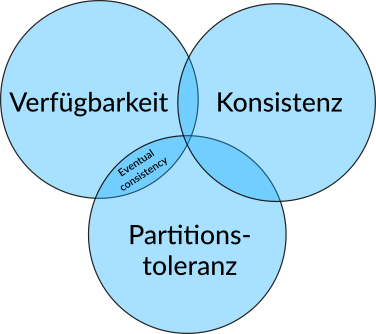
\includegraphics[width=0.6\textwidth]{cap}
  \grayRule
  \caption{Das CAP Theorem}
  \label{fig:cap}
\end{figure}
%
Das System ist besitzt eine hohe Verfügbarkeit wenn alle Anfragen an das System stets beantwortet werden. Die Verfügbarkeit ist gering, wenn die Antwortzeiten des Systems lang sind.
Partitionstoleranz ist gleichzusetzen mit Ausfalltoleranz. Die Datenbank kann auf mehreren Servern verteilt sein. Trotzdem ein Server oder eine Partition ausfällt, kann das System weiterhin funktionieren.\\
Eventual Consistency kommt häufig bei verteilten Datenbanken zur Anwendung und stellt die Konsitenz der Daten nach einem gewissen Zeitfenster sicher (vgl. ~\cite{couchDB} S. 11 ff.). 
% Wenn Verfügbarkeit Priorität hat, können wir Clients die Daten zunächst auf einen Knoten schreiben lassen, ohne darauf zu warten, dass die anderen Knoten synchronisiert werden.
% Wenn die Datenbank weiß, wie sie mit dieser Situation umzugehen hat, sind die Daten irgendwann „letztendlich konsistent“ — allerdings unter Aufgabe der Hochverfügbarkeit der Daten.
% Für viele Anwendungen ist das ein erstaunlich guter Kompromiss.
% Das CouchDB Replikationsmodell erlaubt eine nahtlose, direkte Datensynchronisation zwischen beliebig vielen Geräten.
% Das CouchDB Replikationsprotokoll ist in CouchDB selbst implementiert, das die Serverkomponente abdeckt~\cite{couch}.
%content addressable versions: Idee: Nimm den Objektinhalt (content) und jag ihn durch eine \gls{Hash}funktion\\
%Zuverlässige Synchronisation von Datenbanken auf verschiedenen Geräten.
%Verteilung der Daten über ein Cluster von DB-Instanzen die jeweils einen Teil des requests beantworten (Lastverteilung) und \b{Spiegelung} der Daten über geografisch weit verteilte Standorte.\\
% Durch die inkrementelle (schrittweise) Arbeitsweise kann CouchDB genau dort weitermachen wo es unterbrochen wurde wenn während der Replikation ein Fehler auftritt, beispielsweise durch eine ausfallende Netzwerkverbindung
% \it{Es werden auch nur die Daten übertragen, die notwendig sind, um die Datenbanken zu synchronisieren.}\\
%
%
%Dann gibt es das PouchDB-Projekt, das dasselbe Protokoll in JavaScript implementiert, das auf Browser- und Node.js-Anwendungen abzielt. das deckt Ihre Kunden und dev-Server ab.
%Schließlich gibt es Couchbase Mobile und Cloudant Sync, die auf iOS und Android laufen und das CouchDB Synchronisationsprotokoll in Objective-C bzw. Java implementieren.}\\